\section{Many efficient branches with varying transition energy}
\label{app:exponentialtransition}
This analytical construction sharpens the preceding transition-energy
boundary: at one fixed fleet size, varying compulsory transition energy
can produce many distinct efficient physical pieces. It is an elementary
independent-choice construction with a feasible charging realization, not
a new generic Pareto-complexity or scheduling-hardness claim. No numerical
implementation qualification is asserted.

\begin{proposition}[Efficient pieces at fixed cardinality]
\label{prop:exponentialtransition}
For every $k\ge1$, there is a two-batch charge-only instance with $2k$
services in each batch, fleet cap $2k$, and $2^k$ distinct efficient
physical branches at that same fleet size. Every branch has a corner
that is the unique projected load/cost optimum for some coordinatewise
strictly increasing convex supply objective. The input has polynomial
binary encoding length in $k$; numerical magnitudes grow with $k$.
\end{proposition}

\begin{proof}
Let $w_i=2^i$ for $i=0,\ldots,k-1$, $W=\sum_iw_i$, and choose common
battery capacity $B\ge20\max_iw_i$, for example equality. Block $i$ has
two A services and two B services, with energies $(B/2+3w_i,w_i)$ in
each batch. The allowed graph is the disjoint union of the $k$ complete
$2\times2$ blocks. Within a block, identity edges have transition energy 0
and cross edges have transition energy $6w_i$. No interblock edge or
alternative transition is admitted. A transition is a compulsory task,
not an excursion that may be omitted.

All buses start and end full, with zero reserve, unit efficiency, no V2G
and no other nonservice draw. Use successive windows A$:[0,1]$,
early charging$:[1,2]$, noncharging transition tasks$:[2,3]$,
B$:[3,4]$, terminal charging$:[4,5]$. Tasks have nonnegative consumption
throughout their positive duration. Access is the ideal common-window
access assumed in the two-batch model; no road-metric realization is
claimed. There is one early connector of power/budget
$K=kB/2+4W$ and one terminal connector of power/budget
$H=kB+20W$, with per-bus acceptance at least these powers. A common
fee $f\ge0$ is paid per counted bus.

Each batch has $2k$ simultaneous services and the fleet cap is $2k$.
Thus exactly $2k$ buses are used, every bus serves one service from each
batch, and no singleton or idle bus can compete. Each block chooses its
identity or cross perfect matching. Identity requires early purchase
$6w_i$ and consumes $B+8w_i$ in total. Cross requires zero early purchase
and consumes $B+20w_i$. Indeed each cross duty consumes
$B/2+10w_i\le B$ before terminal charging. The capacity assumption also
ensures each post-early portion fits the battery; it is stronger than
merely checking that condition.

For the set $I$ of identity blocks put
\[
 R=6\sum_{i\in I}w_i,\qquad S_{\max}=kB+20W.
\]
Total consumption is $S_{\max}-2R$, while the sum of early headrooms is
$K$, independent of matching. The per-bus early purchase intervals sum
to $[R,K]$. Thus the \emph{complete} fixed-matching load/cost branch is
\[
 (E,L,c)=(E,S_{\max}-2R-E,2kf),\qquad R\le E\le K.
\]
Every point is physically attained: distribute early purchases within
those intervals and serialize them on the common early connector, perform
the noncharging tasks and services, then serialize the full terminal
refills. Nonnegative consumption and the endpoint battery bounds imply
all intermediate SOC bounds. The interval is nonempty since
$6w_i\le B/2+4w_i$. Terminal purchases are nonnegative and at most $H$.
Conversely every schedule has one of these perfect matchings and exactly
these energy balances, so there are no additional physical branches.

Binary subset sums give $2^k$ distinct values $R=6t$, $0\le t\le W$.
Their corners are $z_R=(R,S_{\max}-3R,2kf)$. For consecutive values
$R<R_{\rm next}$, the portion $R\le E<R_{\rm next}$ is efficient:
larger-requirement branches are unavailable at that early load or a
smaller one, while smaller-requirement branches have a larger terminal
load there. Reducing $E$ on the same branch increases its terminal load.
The final branch is efficient through $E=K$. At $R_{\rm next}$ the new
corner dominates the preceding branch endpoint. Hence these are actual
efficient pieces, not merely differently labelled matchings.

Fix a corner $R_*$ and set $\varepsilon=1/(2\max\{K,1\})$. On the
nonnegative load domain the supply objective
\[
 F_{R_*}(E,L)=3E+L+\varepsilon(E-R_*)^2
\]
is convex and strictly increasing in each coordinate:
$\partial_EF\ge3-2\varepsilon R_*\ge2$ and $\partial_LF=1$.
On a branch indexed by $R$,
\[
 F_{R_*}(E,L)=S_{\max}+2(E-R)+\varepsilon(E-R_*)^2
 \ge S_{\max}.
\]
Equality requires $E=R=R_*$, so that corner is the unique projected
optimum. The constant fleet cost does not affect this conclusion,
including when $f=0$. Different charging allocations with the same loads
can still tie; uniqueness of a literal schedule is not claimed.
\end{proof}

\begin{figure}[ht]
\centering
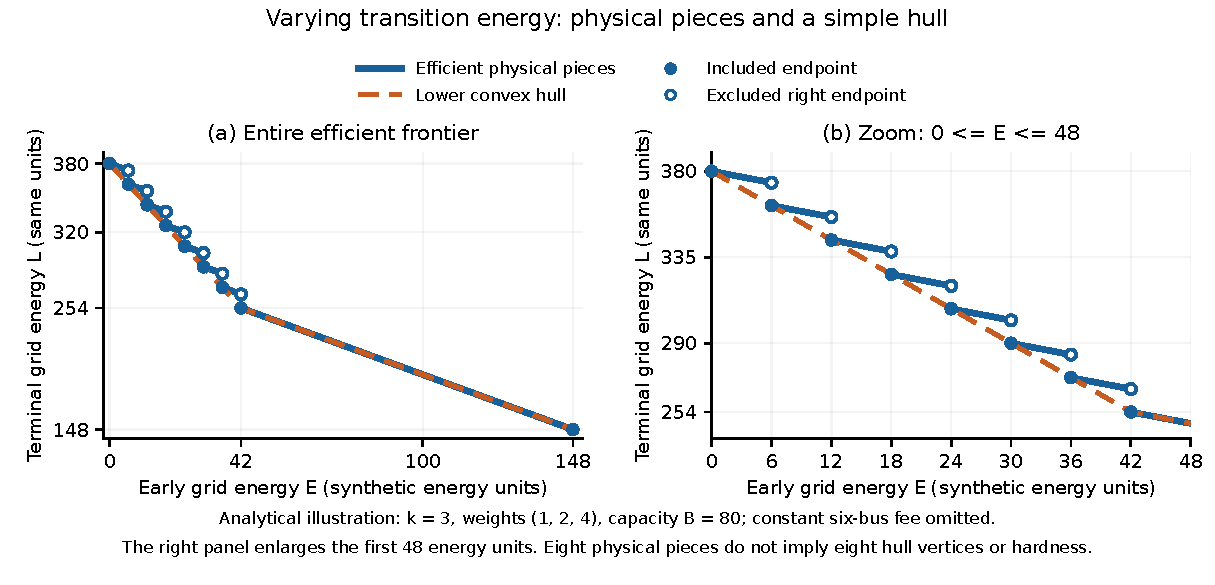
\includegraphics[width=\linewidth]{figures-transition/transition_frontier.pdf}
\caption{The analytical construction with $k=3$, $B=80$, $K=148$ and
$S_{\max}=380$. Its eight efficient physical pieces have collinear corners.
Open circles exclude the dominated right endpoint of each nonfinal piece.
The simple lower hull illustrates why this branch count is not a hull-vertex
or optimization-hardness result. The common six-bus fee is omitted.}
\label{fig:transitionbranches}
\end{figure}

\paragraph{What the branch count does not imply.}
All corners lie on $L=S_{\max}-3E$ and share the supporting price $(3,1)$.
They therefore do not give $2^k$ hull vertices or distinct linear-price
regions: the hull can replace their collinear corners by one edge.
The quadratic term selects a particular projected corner, rather than
making each corner uniquely exposed by a different linear tariff.
Weights, capacity and connector powers grow with this family. Explicit
binary input length is polynomial in $k$, so the explicit physical-piece
count has no polynomial bound in that length; this is not a
$2^{\Omega(\text{input bits})}$ lower bound, a strong-hardness theorem or
an optimization-hardness argument. Indeed $R=6t$, $0\le t\le W$ is a
compact symbolic description. The result neither excludes symbolic
compression nor says this particular family is difficult to optimize.
Its narrow lesson is that one minimum-requirement matching per cardinality
can discard efficient and uniquely convex-optimal projected points when
total energy becomes assignment-dependent.

\begin{corollary}[A support gap with all matching alternatives present]
\label{cor:exponentialgap}
For the complete family in Proposition~\ref{prop:exponentialtransition},
take the smooth, coordinatewise strictly increasing convex supply cost
\[
 F(E,L)=3E+L+\frac{(E-3)^2}{2K}.
\]
For every $k\ge1$ and $f\ge0$, the whole physical and complete-plan
convexified planning values under the stated fleet cap are
\[
 \CH=S_{\max}+2kf,\qquad
 D=\CH+\frac{9}{2K}>\CH.
\]
The hull optimum is unique in projected coordinates. Exactly the physical
corners $R=0$ and $R=6$ minimize physical planning cost. Under
Proposition~\ref{prop:support}, no physical plan is supported at its own
marginal prices in this declared opportunity set.
\end{corollary}

\begin{proof}
Here $K\ge14$, and both corners exist for every $k\ge1$. The Hessian of
$F$ is $\operatorname{diag}(1/K,0)$, and its derivatives on the
nonnegative load domain satisfy $\partial_EF\ge3-3/K>0$ and
$\partial_LF=1$. Every physical branch obeys the affine lower bound
\[
 3E+L=S_{\max}+2(E-R)\ge S_{\max}.
\]
The bound holds on its complete convex hull as well, giving total cost
at least $2kf+S_{\max}+(E-3)^2/(2K)\ge2kf+S_{\max}$.
The equal mixture of the physical corners $(0,S_{\max})$ and
$(6,S_{\max}-18)$ has load $(3,S_{\max}-9)$ and attains equality.
Equality forces that same $E$ and affine bound, so the projected hull
optimum is unique. This argument covers every branch and its convex
mixtures, not just the two used by the upper witness.

On a physical branch total cost equals
\[
 2kf+S_{\max}+2(E-R)+\frac{(E-3)^2}{2K}.
\]
Its derivative in $E$ is at least $2-3/K>0$, so it is minimized at
$E=R$. Among $R=6t$, $0\le t\le W$, exactly 0 and 6 are nearest to 3,
at distance 3. Their objective excess is therefore $9/(2K)$, establishing
the stated physical value and its two minimizing projected corners.
All plans have the same fee, including when $f=0$. The strict gap and
the classical support criterion give the final assertion.
\end{proof}

This is a whole-opportunity-set example: its $2^k$ efficient matching
alternatives are all admitted, and the fleet cap excludes singleton or
extra-bus escape routes. Having many additional feasible alternatives
therefore does not by itself guarantee restoration of own-marginal-price
support. It is not a claim that every expansion preserves a gap. The
exact gap $9/(2K)$ shrinks as $K$ grows; there is no uniform lower bound,
prevalence, operational-routing or hardness conclusion. The common
supporting price $(3,1)$ at the hull optimum and the simple hull remain
consistent with the earlier collinearity and compression caveats.

% Proposed body paragraph (not wired):
% Varying transition energy can create more than an isolated discarded
% branch: Appendix~\ref{app:exponentialtransition} constructs a fixed-fleet
% two-batch family with 2^k distinct efficient physical pieces, each with
% a uniquely convex-optimal projected corner. All corners share one linear
% supporting price, however, and admit a compact symbolic description.
% This illustrates the loss of the single-statistic physical reduction,
% not exponential hull complexity, computational hardness or a new generic
% multiobjective result.
